\chapter[Metodologia]{Metodologia}

Neste capítulo, serão apresentados detalhes da metodologia aplicada no desenvolvimento teórico e prático do trabalho. Neste sentido, as atividades de pesquisa são classificadas conforme a abordagem, natureza, objetivos e procedimentos. Além disso, é definida a sequência de atividades realizadas neste trabalho de conclusão de curso, detalhando a metodologia e os processos envolvidos no desenvolvimento do \textit{software}, além dos aspectos metodológicos estabelecidos com base na análise dos resultados obtidos. Por fim, exibe-se o cronograma de atividades. 

\section{Metodologia de Pesquisa}
\label{sec:met_pesquisa}
De acordo com \citeauthoronline{gerhardt2009metodos} (\citeyear{gerhardt2009metodos}), a Metodologia pode ser classificada como o estudo da organização, dos caminhos a serem trilhados, para se realizar uma pesquisa ou um estudo, ou para produzir ciência. Já a pesquisa científica, refere-se ao resultado de “um inquérito ou exame minucioso, realizado para resolver um problema, recorrendo a procedimentos científicos” \cite{gerhardt2009metodos}.

A partir das definições de \citeauthoronline{gerhardt2009metodos} (\citeyear{gerhardt2009metodos}), esta seção visa categorizar a pesquisa deste trabalho quanto à abordagem, à natureza, aos objetivos e aos procedimentos.

\subsection{Abordagem da Pesquisa}
As pesquisas utilizadas neste trabalho podem ser classificadas como Qualitativas e Quantitativas. A pesquisa qualitativa visa obter uma compreensão mais profunda de um grupo social, de uma organização, entre outros. Portanto, a pesquisa qualitativa, preocupa-se com aspectos da realidade que não podem ser quantificados, concentrando-se em compreender e explicar a dinâmica das relações sociais. Já a pesquisa quantitativa se centra na objetividade, tendo o objetivo de enfatizar o raciocínio dedutivo, as regras da lógica e as propriedades mensuráveis da experiência humana \cite{gerhardt2009metodos}.

\subsection{Natureza da Pesquisa}
A pesquisa deste trabalho pode ser classificada como Aplicada. A pesquisa aplicada visa produzir conhecimento para aplicação prática, de modo a resolver problemas específicos. Por outro lado, a pesquisa básica visa gerar conhecimentos novos, sem aplicação prática prevista \cite{gerhardt2009metodos}.

\subsection{Objetivos da Pesquisa}
Como objetivo, a presente pesquisa classifica-se como Exploratória. A pesquisa exploratória consiste em proporcionar maior familiaridade com o problema, visando torná-lo mais explícito ou formular hipóteses \cite{gil2002elaborar}.

\subsection{Procedimentos}
A pesquisa deste trabalho pode ser classificada como Bibliográfica e Pesquisa-Ação. A pesquisa bibliográfica é realizada a partir de um acervo de referências teóricas analisadas e publicadas por meios escritos e tecnológicos, como livros, artigos científicos, \textit{sites}, entre outros. A pesquisa-ação, por outro lado, pressupõe a participação planejada do pesquisador na situação problemática a ser investigada, visando diagnosticar um determinado problema sobre uma dada situação, para chegar em um resultado prático \cite{gil2002elaborar}.

\section{Fluxo de Atividades}

\label{sec:fluxo_atividade}
    
Para a construção deste trabalho, foram seguidas algumas etapas que viabilizaram o bom andamento deste trabalho. Para melhorar a visualização e evidenciar essas etapas, foram elaborados os diagramas \ref{fig:bpmn_geral}, a partir da notação \textit{BPMN}\footnote{Notação gráfica criada pelo grupo conhecido como \textit{BPMI} no ano de 2002 para representação de processos de negócio}.

\begin{figure}[H]
    \begin{center}
        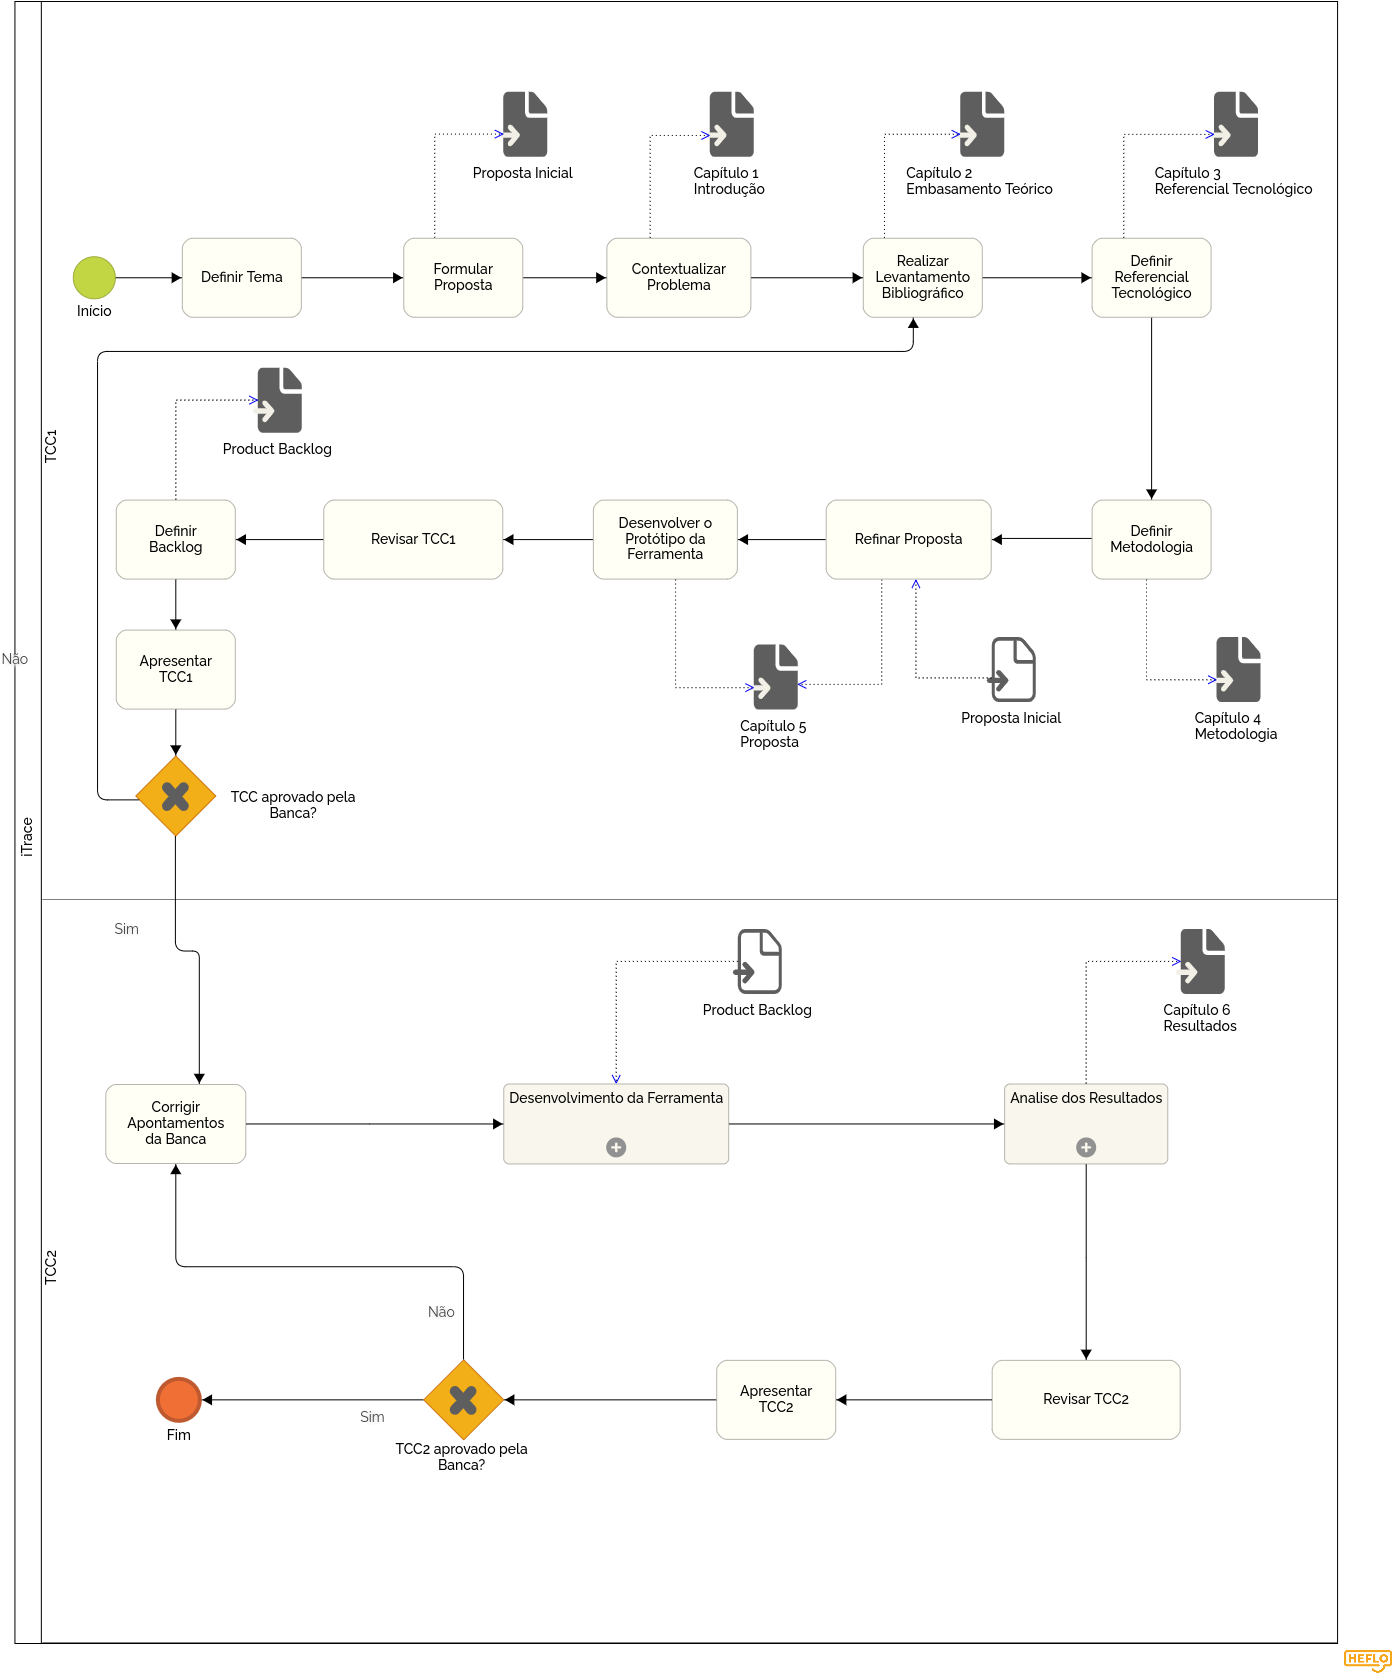
\includegraphics[scale=0.25]{figuras/Metodologia/bpmn_geral.png}
        \caption{{Diagrama BPMN da metodologia. Fonte: Autores, 2022}}
        \label{fig:bpmn_geral}
    \end{center}
\end{figure}

\begin{enumerate}
    \item \textbf{Definição do tema}: atividade destinada à escolha do tema para o desenvolvimento da monografia. Foram apresentados diversos temas aos orientadores de interesse e, após várias discussões, foi escolhido o tema com maior perspectiva de desenvolvimento e interesse entre as partes, a ferramenta \textit{iTrace};
    \item \label{item:proposta} \textbf{Formulação da proposta}: esta etapa consiste em definir as atividades para determinar e contextualizar o escopo, objetivos e justificativas deste trabalho;
    \item \textbf{Contextualização do problema}: sabendo do problema e da proposta, essa atividade consistiu em tomar um panorama amplo da área e do seu contexto;
    \item \textbf{Revisão bibliográfica}: elaborada a formulação, o passo mais importante foi a revisão do que já foi publicado na literatura da área que a dupla se propôs atuar;
    \item \textbf{Definição do suporte tecnológico}: tendo embasado a parte teórica do trabalho, esse passo se propôs a definir o ferramental e as tecnologias necessárias para poder viabilizar este trabalho;
    \item \textbf{Definição da metodologia}: esta atividade, de suma importância, foi o momento, em que a dupla dedicou-se em desenhar um modelo que viabilizasse a execução de todo o trabalho, olhando e esquematizando o que já havia sido realizado e definindo os passos que ainda estariam por vir;
    \item \textbf{Refinar e detalhar proposta}: a partir da proposta definida no passo \ref{item:proposta}, a mesma foi melhorada e refinada, a partir das orientações obtidas e novos rumos dados pelas atividades anteriores;
    \item \textbf{Desenvolvimento do Protótipo da Aplicação}: para podermos ilustrar e viabilizar a ferramenta \textit{iTrace}, foi feito um protótipo de alta fidelidade visando demonstrar a aplicação para a banca. Realizando, também, o papel de uma prova de conceito;
    \item \textbf{Revisão e refinamento sistemático do TCC 1}: concluindo todos os passos necessários para a construção do documento a partir dos requisitos do TCC 1, esta atividade dedica-se a revisar, de forma sistemática, todos os pontos elencados verificando sua acuidade;
    \item \label{item:revision} \textbf{Apresentação do TCC 1}: atividade destinada à validação dos professores Doutores do trabalho desenvolvido;
    \item \textbf{Refinamento e apontamentos da banca}: a partir dos \textit{feedbacks} dados pelos professores da banca, realizar a revisão e aperfeiçoamento do documento;
    \item \textbf{Definição do \textit{Product Backlog}}: para iniciar o desenvolvimento da ferramenta, esta atividade é essencial para elencar, clara e objetivamente, os passos necessários para a construção do sistema proposto;
    \item \textbf{Desenvolvimento da Aplicação}: este subprocesso consiste na atividade de desenvolvimento da ferramenta que está melhor detalhado na figura \ref{fig:bpmn_dev}. As subatividades serão explicadas na seção \ref{sec:met_dev}, em que define a metodologia de desenvolvimento deste trabalho;
    \item \textbf{Análise dos Resultados}: para validar o funcionamento da ferramenta, testes com usuários reais serão aplicados de modo a verificar se a ferramenta possibilita o desenvolvimento do processo da Engenharia de Requisitos;
    \item \textbf{Revisão e refinamento sistemático do TCC 2}: consiste na mesma atividade do item \ref{item:revision}, mas no escopo do TCC 2, e
    \item \textbf{Apresentação do TCC 2}: apresentação final da aplicação em funcionamento com os resultados obtidos a partir dos testes realizados com os usuários validados pela banca de professores.
\end{enumerate}

\section{Metodologia de Desenvolvimento}

No que tange a metodologia voltada ao desenvolvimento prático da ferramenta, por afinidade da dupla, foi escolhida a metodologia \textit{Scrum} aliada ao \textit{Kanban}.

O \textit{Scrum} é uma metodologia ágil para desenvolvimento de produtos complexos que mudam os requisitos rapidamente. O seu desenvolvimento é dado por uma série de iterações chamadas \textit{Sprint}, que no caso do nosso projeto, serão semanais. A cada \textit{Sprint} é realizada uma reunião de planejamento (\textit{Sprint Planning}) e de revisão do trabalho (\textit{Sprint Review \& Restrospective}), com foco na melhoria contínua do processo e iteração entre as pessoas. Para promover a transparência e o alinhamento do trabalho, usaremos dois artefatos, o \textit{Backlog} do Produto(Product Backlog) e o \textit{Backlog} da \textit{Sprint} (Sprint Backlog), onde cada um descreve o trabalho a ser realizado, respectivamente, no produto e na \textit{Sprint} \cite{carolipaulo2021}.

O \textit{Kanban}, por outro lado, é uma metodologia que visa um alinhamento mais claro de uma equipe, além de dar visibilidade ao que está sendo elaborado, proporcionando um ambiente favorável a uma comunicação com o menor ruído possível. Além disso, garante uma carga de trabalho adequada, considerando a capacidade produtiva da equipe. Um ponto essencial dessa metodologia é o quadro que deixa as tarefas e seu status visível para todo o time, pontuando em qual parte do fluxo de trabalho esta tarefa está \cite{K_Condensed}.

\subsection{Processo de Desenvolvimento}

\label{sec:met_dev}

O processo de desenvolvimento escolhido pode ser visualizado na imagem \ref{fig:bpmn_dev}, elaborado na notação \textit{BPMN} a partir do detalhamento do subprocesso \textbf{Desenvolvimento da Aplicação} da imagem \ref{fig:bpmn_geral}, e consiste nas seguintes etapas:

\begin{figure}[H]
    \begin{center}
        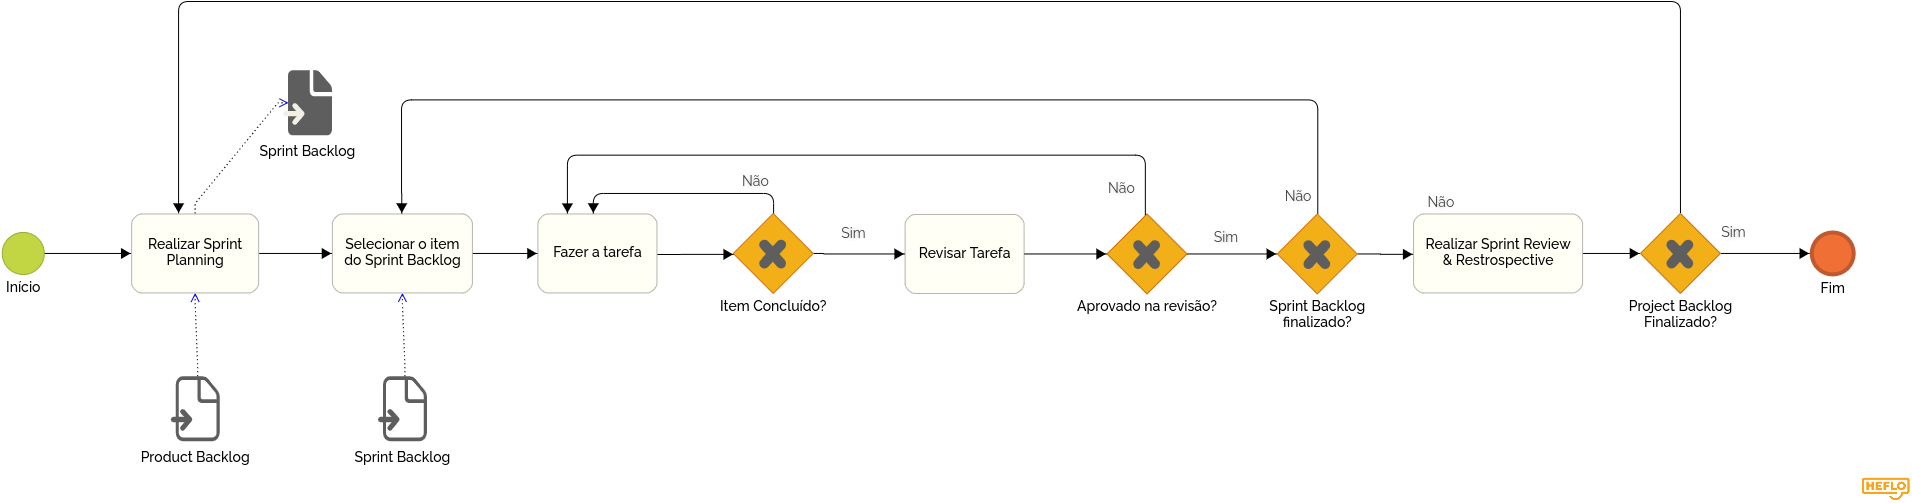
\includegraphics[scale=0.23]{figuras/Metodologia/bpmn_dev.png}
        \caption{{Diagrama BPMN de desenvolvimento. Fonte: Autores, 2022}}
        \label{fig:bpmn_dev}
    \end{center}
\end{figure}

\begin{enumerate}
    \item \textbf{\textit{Sprint Planning}}: a partir do \textit{Product Backlog}, as atividades são selecionadas consoante a sua prioridade e pontos definidos para execução da mesma. As tarefas selecionadas consideram a capacidade produtiva da dupla na \textit{Sprint} e gerenciamento de riscos para a entrega do produto;
    \item \textbf{Selecionar o \textit{item} do \textit{Sprint Backlog}}: A partir do \textit{Sprint Backlog}, as tarefas são selecionadas para serem executadas pela dupla;
    \item \textbf{Fazer a tarefa}: consiste em desenvolver a tarefa selecionada;
    \item \textbf{Revisar tarefa}: consiste no processo de revisão pela pessoa contrária da dupla que a desenvolveu, para verificar se os padrões de desenvolvimento da comunidade foram seguidos, e se atende com o que foi definido no \textit{Product Backlog};
    \item \textbf{\textit{Sprint Review \& Restrospective}}: com a conclusão da \textit{Sprint}, essa atividade elenca os pontos positivos e negativos da \textit{sprint}, além de revisar as atividades entregues.
\end{enumerate}


\section{Metodologia de Análise de Resultados}

Como definido na Seção \ref{sec:met_pesquisa}, o método orientado para o processo de análise dos resultados do trabalho será a Pesquisa-Ação. De acordo com \citeauthoronline{gil2002elaborar} (\citeyear{gil2002elaborar}), a pesquisa-ação ocorre com muitas oscilações entre as fases, determinada pela dinâmica do grupo de pesquisadores em seu relacionamento com a situação pesquisada. Além disso, a pesquisa-ação apresenta uma série de ações desordenadas no tempo considerando os seguintes passos: a) fase exploratória; b) formulação do problema; c) construção de hipóteses; d) realização do seminário; e) seleção da amostra; f) coleta de dados; g) análise e interpretação dos dados; h) elaboração do plano de ação; e i) divulgação dos resultados.

Portanto, a pesquisa-ação deste trabalho passará pelas seguintes etapas:

\begin{itemize}
    \item \textbf{Coleta de dados}: nesta etapa, realiza-se a coleta de dados quantitativos por meio da ferramenta desenvolvida e qualitativos através da interação dos usuários com a ferramenta;
    \item \textbf{Análise e interpretação dos dados}: nesta etapa, busca-se examinar os dados coletados e, em seguida, realizar a explanação dos resultados adquiridos;
    \item \textbf{Elaboração do plano de ação}: pretende-se elaborar um plano de ação que visa mitigar os problemas encontrados a partir dos dados analisados, e 
    \item \textbf{Divulgação dos resultados}: para validação, os resultados obtidos e o plano de ação definido, será validado com a banca de mestres e doutores para verificar a adequação da aplicação no escopo de atuação.
\end{itemize}

A primeira investigação será voltada a testes com os \textit{stakeholders} que avaliam a experiência do usuário na ferramenta, de forma que valide se a ferramenta cumpre com os \textbf{objetivos específicos} \ref{oe_guiar_usuario} e \ref{oe_ux_facilitada}. Em seguida, serão realizados testes que busquem validar se os requisitos propostos foram cumpridos e, principalmente, se o \textbf{objetivo específico} \ref{oe_mvp} foi satisfeito.

\section{Cronogramas}

As Tabelas \ref{tab:cronograma_tcc1} e \ref{tab:cronograma_tcc2} apresentam os cronogramas do TCC 1 e 2, respectivamente. Nas tabelas, as atividades são descritas de acordo com suas datas de implementação, baseando-se no fluxo de atividades descrito na Seção \ref{sec:fluxo_atividade}.

\begin{table}[H]
    \centering
    \scalebox{0.9}{%
    \begin{tabular}{l*{4}{c}r}
        \hline
        Atividade & Jan/2022 & Fev/2022 & Mar/2022 & Abr/2022 \\
        \hline
        Definição do Tema & X & & & \\
        Formulação da Proposta & & X & & \\
        Contextualização do Problema & & X & & \\
        Revisão Bibliográfica & & & X & \\
        Definição de Suporte Tecnológico & & & X & \\
        Definição da Metodologia & & & & X \\
        Refinar e Detalhar Proposta & & & & X \\
        Desenvolvimento do Protótipo da Aplicação & & & & X \\
        Revisão e Refinamento sistemático do TCC & & & & X \\
        Apresentação do TCC 1 & & & & X \\
        \hline
    \end{tabular}}
    \caption{Cronograma de Atividades do TCC 1}
    \label{tab:cronograma_tcc1}
\end{table}

\begin{table}[H]
    \centering
    \scalebox{0.8}{%
    \begin{tabular}{l*{5}{c}r}
        \hline
        Atividade & Mai/2022 & Jun/2022 & Jul/2022 & Ago/2022 & Set/2022 \\
        \hline
        Refinamento e apontamentos da Banca & X & & & & \\
        Definição do \textit{Product Backlog} & X & & & & \\
        Desenvolvimento da Aplicação & X & X & X & X & \\
        Análise dos Resultados & & & & X & X \\
        Revisão e refinamento sistemático do TCC & & & & & X \\
        Apresentação do TCC 2 & & & & & X \\
        \hline
    \end{tabular}}
    \caption{Cronograma de Atividades do TCC 2}
    \label{tab:cronograma_tcc2}
\end{table}